\chapter{Проектирование}
\label{cha:ch_1}

\section{Исследование распространённости использования класса Input}
Имея перед собой цель создания ассетов способных автоматизировать действия разрабатываемого приложения, было принято решение о том, что в качестве основного способа запрашивания ввода необходимо было взять класс Input из стандартной библиотеки платформы \textit{Unity} как наиболее лёгкий для использования.

Критерием лёгкости использования способов запрашивания ввода здесь является минимальное количество необходимых единиц компиляции (ЕК) и количество использованных строк кода (ИСК). Согласно официальному мануалу посвящённому системам запрашивания ввода \cite{unity_input_systems} в платформе \textit{Unity} существует два модуля подобных систем: Input Manager и Input System. Первая система включает в себя два способа: Класс Input и интерфейсы-маркеры. Вторая система по-сути своей является альтернативой первой, она поставляется отдельно и требует установки дополнительных зависимостей.

\begin{table}[H]
	\caption{\label{tab:bolts}Количество ЕК и ИСК на способ запрашивания ввода}
	\begin{center}
		\begin{tabular}{|c|c|c|}
			\hline
			& \multicolumn{2}{c|}{Количество} \\
			\cline{2-3}
			\raisebox{1.5ex}[0cm][0cm]{Способ запрашивания ввода}
			& ЕК & ИСК \\
			\hline
			Класс Input & 3 & 1 \\
			\hline
			Интерфейсы-маркеры & 10 & 1 \\
			\hline
			Input System & 10 & 1 \\
			\hline
		\end{tabular}
	\end{center}
\end{table}

Утверждение: Input - популярен, т.е Input - распространён,
распространённость = мат ожидание ген совокупности больше 0
ген совокупность: множество чисел означающих количество использований класса Input в кодовой базе проекта который либо самый релевантный по запросу (проект на Unity), имеет больше всего звёзд, имеет больше всего форков, самый живой - причиной именно такого выбора фильтров поиска является тот факт, что по-сути в выбранных проектах используются самые распространённые и удобные практики, т.е по 1 ому такому проекту можно судить, что глядя на него другие разрабы тоже поступают также, ведь выбранный проект весьма жив и успешен.
источник данных GitHub

Выбран интервальный критерий бутстрапа с параметрами: уровень значимости 0.1, количество повторных выборок 99509 - равный количеству всех найденных проектов на юнити на гитхабе, длина выборки 3970 = максимальное количество данных которых удалось извлечь

\begin{figure}[H]
	\centering
	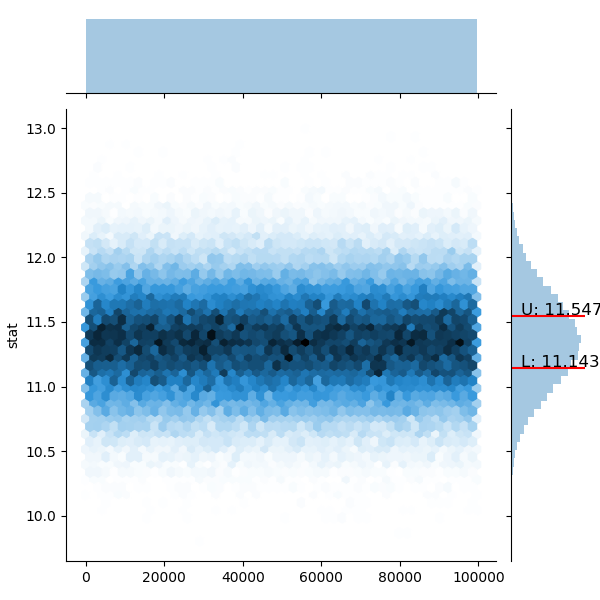
\includegraphics[width=\linewidth]{experiment.png}
	\caption{Диаграмма рассеивания бутстраповской интервальной оценки}
	\label{experiment}
\end{figure}

\section{Класс совместимых приложений}
Разработанная в рамках данной работы группа ассетов имеет название Automated Test Framework (ATF) и может быть интегрирована c любым  \textit{Unity}-проектом, система ввода которого построена вокруг класса из стандартной библиотеки \textit{Unity} по взаимодействию с вводом Input. Под это описание подходит большая часть \textit{Unity}-приложений и в этом выражена универсальность предложенного решения. Ранее среди свободных для использования ассетов не было представлено решений для автоматизации ни success-тестов, ни тестирования главного потока сценария использования, ни других подходов для функционального тестирования приложений, кроме как через механизмы стандартного пакета unit-тестирования \textit{Unity}. Однако как бы ни был хорош подход использования инструментария unit-тестирования, для того чтобы покрыть все возможные сценарии действий внутри проекта, пришлось бы либо писать свой модуль тестов под каждый из аспектов, либо же на его основе реализовывать сложную универсальную систему.

\section{Определение теоретической базы}

\begin{itemize}
	\item 
	создание расширяемой базы кода, которая бы отвечала всем требованиям принципов SOLID \cite{solid}, DRY \cite{dry} и принципа бритвы Оккама \cite{razor},
	\item
	компоновка решения в множество ассетов для легкой переносимости результирующего продукта, 
	\item а также  обеспечение интеграции в код уже написанных продуктов.
\end{itemize}


\begin{figure}[H]
	\centering
	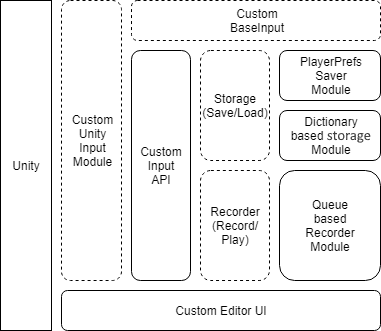
\includegraphics[width=0.7\linewidth]{platform.png}
	\caption{Диаграмма платформы решения}
	\label{platform}
\end{figure}

На этапе проектирования была составлена диаграмма платформы (см. рис. \ref{platform}), каждый блок которой -- это изолированная группа методов API, решающая свои задачи: 
\begin{itemize}
	\item \textit{Unity} -- непосредственно сам игровой движок;
	\item \textit{Custom Unity Input Module} -- абстракция, объединяющая управление вводом;
	\item \textit{Custom Input API} -- собственно API, который вызывает нативные методы по запросу ввода;
	\item \textit{Custom BaseInput} --  сущность, которяа является реализацией объекта обработки потока данных через мост (Bridge), объединяя статичные методы по перехвату/симуляции ввода и обернутые события (Events);
	\item \textit{Storage} --  абстракция, отвечающая за функционал хранения и манипуляции записанных действий;
	\item \textit{Recorder} -- абстракция, отвечающая за запись действий;
	\item \textit{Custom Editor UI} -- система пользовательских окон для управления всеми процессами;
	\item \textit{PlayerPrefs Save/Load Module} -- система реализации абстракции модуля по сохранению/загрузке записанных действий на базе стандартного класса PlayerPrefs;
	\item \textit{Dictionary based Module} -- реализация абстракции хранилища записанных действий, основанная на структуре данных ``Словарь'';
	\item \textit{Queue based Recorder Module} -- реализация абстракции, отвечающей за запись действий, основанная на структуре данных ``Очередь''.
\end{itemize}

Для выполнения поставленных задач было разработано решение, являющееся, по своей сути, модифицированным адаптером, который перехватывает и симулирует ввод. Для его эффективной реализации стало органичным использовать несколько архитектурных паттернов:
\begin{itemize}
	\item
	\textit{Interceptor} -- шаблон для перехвата и подмены входных данных с периферийных устройств \cite{interceptor};
	\item
	\textit{Broker} -- шаблон для интеграции и взаимодействия с встроенной системой управления входными данными \textit{Unity} \cite{broker};
	\item
	\textit{PAC (Presentation–abstraction–control)} -- шаблон для организации взаимодействия зависимых систем \cite{pac}.
\end{itemize}

Для подмены стандартного класса Input был создан перехватчик ATFInput (см. рис. \ref{atfInput}), который наследуется от стандартного класса BaseInput для использования встроенной пользовательской системы управления вводом. ATF -- это сокращение от английского Automated Test Framework, которое переводиться как: фреймворк автоматизированного тестирования. Так как класс Input содержит в себе только статичные методы, декорация их для перехвата внутри ATFInput позволила совместить и классический перехват ввода и облегчить в дальнейшем перехват событий ввода. Иначе говоря, было проведено совмещение перехватчика для класса Input и класса BaseInput  для взаимодействия с событиями ввода внутри \textit{Unity}. 

\begin{figure}[H]
	\centering
	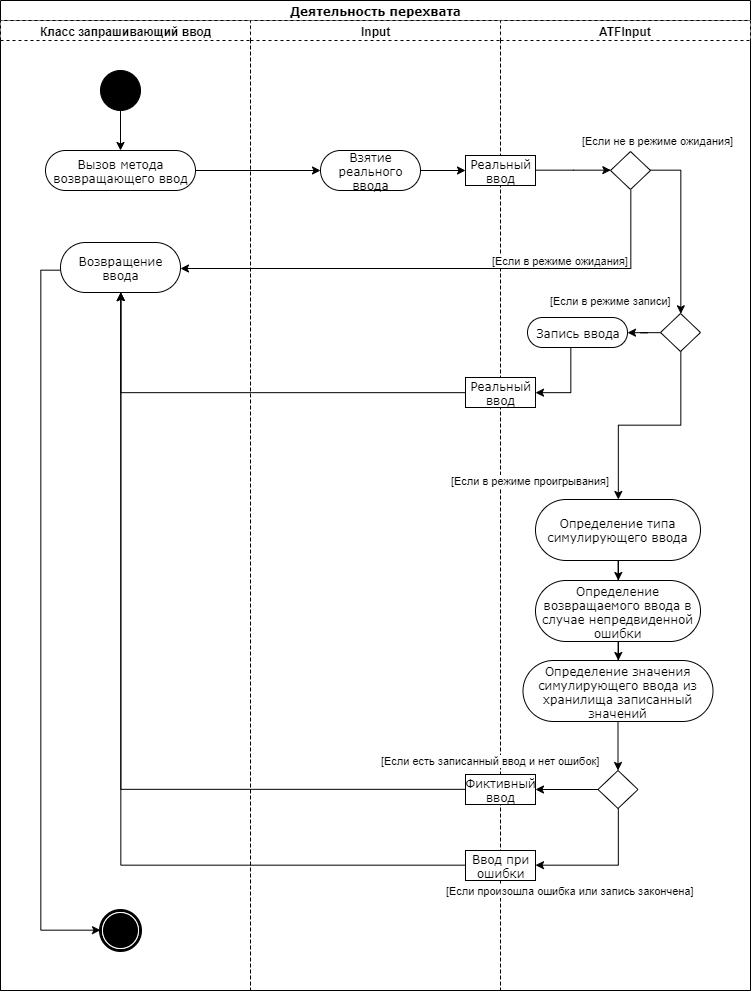
\includegraphics[width=\linewidth]{atfInput.png}
	\caption{Диаграмма деятельности ATFInput}
	\label{atfInput}
\end{figure}


Для интерпретации (проигрывания) первоначально использовался паттерн Interpreter с терминалами ожидания внутри Coroutine. Однако после попытки тестовой реализации данного шаблона был произведен отказ от этого шаблона в пользу метода записи, основанного на структуре данных ``Очередь'', так как для правильной работы терминалов ожидания необходимо было просчитывать заранее действия пользователя, что затруднительно.